\documentclass[11pt,a4paper]{article}
\usepackage[utf8]{inputenc}
\usepackage[catalan]{babel}
\usepackage{amsmath}
\usepackage{amsfonts}
\usepackage{amssymb}
\usepackage{graphicx}
\usepackage[left=4cm,right=4cm,top=4cm,bottom=4cm]{geometry}


\begin{document}
\title{Millora de rendiment d'un sistema d'avaluació de traductors automàtics}
\author{Ibai Gilabert Rodríguez}
\date{20 de març de 2015}
\maketitle
\newpage

\begin{abstract}
Informe de seguiment del TFG "Millora de rendiment d'un sistema d'avaluació de traductors automàtics".
\\

Autor: \textit{Ibai Gilabert Rodríguez}

Director: \textit{Jordi Turmo Borras}

Codirectora: \textit{Meritxell González Bermúdez}
\end{abstract}
\newpage

\tableofcontents
\newpage

\section{Introducció}

El camp de la traducció automàtica i, en definitiva, el tractament del llenguatge natural està en alça. La seva rellevància augmenta dia a dia, en la mesura que la nostra capacitat tecnologia creix els horitzons en aquesta àrea són cada vegada més i més enlluernadors.
\\

L'objectiu d'aquest projecte és fer-ho real. És aprofitar tota la capacitat tecnològica de la que disposem de manera que esdevingui el NLP \textit{(Natural language processing)} una empresa més tractable. En concret com avaluar traductors automàtics. Tasca especialment conflictiva ja que fins i tot diferents humans poden estar en desacord en decidir si una traducció és correcte o no.
\\

El NLP és \textit{per se} molt complex computacionalment parlant. Requereix de molts recursos, principalment temps i memòria, el que implica haver de disposar d'entorns d'execució d'altres prestacions.
\\

\subsection{Context}
Prenem com a \textit{baseline} un sistema plenament funcional: ASIYA\cite{asiya}.
\\

A continuació definim breument els ítems amb els que treballa ASIYA. 

\paragraph{Input} Conjunt de documents agrupats en 3 categories diferents: \textit{source} (conjunt de documents en llengua origen), \textit{reference} (traduccions humanes associades a cada \textit{source} en llengua destí) i \textit{system} (traduccions automàtiques en llengua destí de cada document per a cada traductor automàtic dins d'un conjunt de traductors automàtics). Aquests inputs poden venir donats en diferents formats. ASIYA els adaptarà per tractar-los en format text.

\paragraph{Output} ASIYA generarà una puntuació \textit{(score)} per a cada sistema i cada mètrica amb 3 nivells de granularitat: segment (oració), document i sistema. Aquests \textit{scores} es desaran en fitxers comprimits amb la finalitat de no repetir càlculs en execucions posteriors.
\\

A més, entre els paràmetres de configuració estan les mètriques que voldrem executar. Aquestes mètriques es poden agrupar en "families" o \textit{metric sets} per a millor confort.
\\

ASIYA és una eina que posa a disposició un ventall molt ampli i heterogeni de mètriques d'avaluació i meta-avaluació, la majoria d'elles són usables i perfectament vàlides per a ser executades de manera singular. Així que ASIYA actua més aviat com una interfície per tota aquesta amalgama de mètriques. El principal problema és la ineficiència. Aquesta ineficiència procedeix del comput seqüencial de càlculs molt lents i amb requeriments de memòria dispars.
\\

En l'actualitat no hi ha cap sistema, per quantitat i qualitat, com ASIYA, com a mínim d'aquestes característiques. No obstant, el seu principal handicap són els recursos que exigeix. Tot i que algunes mètriques fan us d'eines externes com ara processadors lingüístics que, per motius de manteniment i flexibilitat no toquem i tractem com a caixes tancades i completament opaques, sí és cert que es deixa entreveure una certa concurrència en el càlcul dels \textit{scores}, derivat de fragmentar els inputs. Així com també és concurrent l'execució de moltes mètriques ja que la majoria són completament independents. 
\\

És a dir, concurrència a nivell de mètrica i concurrència a nivell de document.
\\

Aquí és on el projecte agafa sentit. Com podem fragmentar l'execució d'ASIYA de manera que mitjançant alguna arquitectura paral·lela millorem l'ús dels recursos?
\\

\subsection{Abast}
Com ja s'ha esmentat ASIYA és una eina flexible, adaptable i de fàcil integració. Això és una característica que no volem perdre.  Això vol dir que les tasques de manipulació de l'eina com afegir mètriques, llengües; modificar formats, etc han de ser el més fàcils possible. Es persegueix una filosofia o idea de senzillesa en el seu ús i edició. Adaptabilitat al cap i a la fi.
\\

Així doncs si no volem modificar el còmput, el que ens queda es modificar les dades. Com a primera presa de contacte podem definir el nostre enfoc de la següent manera: si tenim una entrada de mida $N$ la partirem en $n \in N$, fragments perquè ASIYA pugui executar els $n \in N$ fragments de manera paral·lela, aquesta és la idea.
\\

Per portar-ho a terme, es plantejarà un re-disseny íntegre de tot el sistema. Aquest serà en un llenguatge més adient per a les nostres necessitats (eficiència i concurrència). S'ha escollit \texttt{C++} per la seva estructura de classes, tipificació i compatibilitat amb diferents paradigmes de programació paral·lela que veurem més endavant.

\newpage
\section{Estat de l'Art}

\subsection{Models de computació paral·lela}

\subsubsection{Clúster de computació}
Mastodòntics és un bon adjectiu per a descriure els recursos que molts procediments de tractament del llenguatge natural exigeixen. Ja s'ha comentat la necessitat d'un entorn d'execució d'altes capacitats. Per aquestes tasques de recerca i altres l'any 2010 va néixer el \textit{Laboratori de Recerca i Desenvolupament} (RDlab). Aquest ofereix un entorn ideal per a les nostres necessitats: \textit{"El nostre clúster de computació d'altes prestacions (HPC) proporciona un entorn perfecte per execucions massives"}\cite{cluster}
\\

Aquest sistema implementa un \textit{Sun Grid Engine}. El clúster el composen una seguit de nodes (independents entre ells i absolutament autònoms). Cadascun d'aquests nodes disposa d'uns recursos hardware variable i en constant actualització. Per fer ús del sistema els usuaris envien tasques \textit{(jobs)} i aquest les encua i les enviarà a executar seguint una sèrie de paràmetres (disponibilitat, prioritat, etc) als nodes que s'escaiguin.
\\

Aquest mecanisme ens permet executar \textit{jobs} amb els quals crear altres \textit{jobs} que idealment s'executaran de manera paral·lela (el sistema de cues s'encarregarà de la planificació de recursos). 
\\

Entenent que és de menester un sistema HPC i essent aquesta la millor opció que tenim al nostre abast, aprofitarem aquesta tecnologia amb la intenció d'implementar el paral·lelisme que desitgem. 

\subsubsection{\textit{GPU Computing}}
En un inici, el paradigma de computació paral·lela en GPU va ser ideat per a resoldre una necessitat impresiosa de càlcul cada vegada més massiu amb l'objectiu de produir gràfics més realistes. Aquesta motivació es veu reflectida en l'arquitectura. Totes les GPUs comparteixen un filosofia de disseny orientada a solucionar càlculs molt repetitius de manera massiva propis del món gràfic.
\\

\begin{figure}[hbtp]
\centering
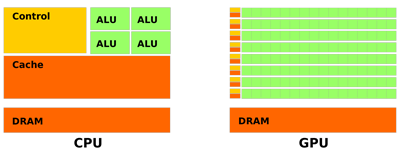
\includegraphics[width=10cm]{resources/cpu-gpu_w.png}
\caption{CPU-GPU, conceptes diferents}
\end{figure}

Entrant una mica més a fons en l'arquitectura GPU, el detall que, d'entrada pot provocar certa perplexitat, és el nombre de nuclis que conté. És una qualitat característica que a priori pot semblar  miraculosa\footnote{Una GPU de gamma mitja actual sobrepassa els 1000 \textit{cores}.}. Cal destacar que no són \textit{cores} en el sentit clàssic del vocable informàtic (unitats de propòsit general, amb unitat de control, entrada/sortida, etc). Aquests nuclis s'assemblen més aviat a ALUs \textit{(Arithmetic Logic Unit)}. És a dir, a petits coprocessadors destinats exclusivament al càlcul numèric.
\\

La història de com aquestes unitats van transcendir l'àmbit gràfic per constituir-se com a alternativa real per a programes de propòsit general  és molt interessant. Els exemples més recurrents són aplicacions científiques en l'àmbit de la recerca (bioinformàtica, química computacional..), i també empresarial (simulació de fluids, etc)\cite{CUDAapplications}. De fet, els principals fabricants, especialment NVIDIA, ja fa anys que presenten solucions d'altes prestacions no orientades al \textit{rendering}.  Es poden aconseguir resultats de super-computador de petita escala en un ordinador personal.
\\

\begin{figure}[hbtp]
\centering
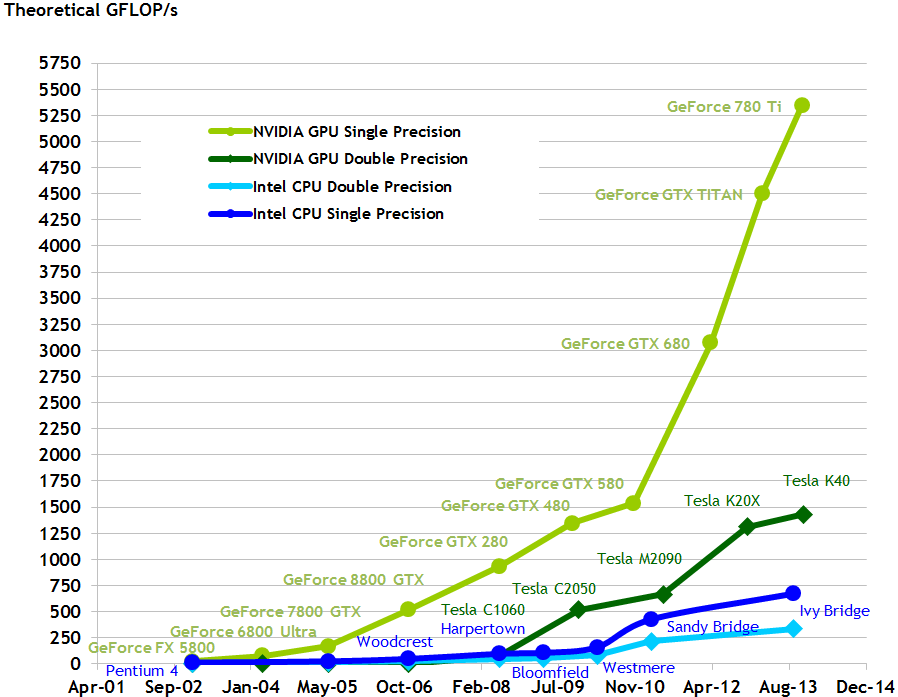
\includegraphics[width=12cm]{resources/floating-point-operations-per-second.png}
\caption{Comparativa de rendiment en \textit{FLOPS}}
\end{figure}

NVIDIA presenta una gamma de GPUs dedicada al segment de la supercomputació anomenada "Tesla"\cite{tesla}.
\\

Pel que fa a la programació amb GPUs, existeixen vàries plataformes: algunes lliure com OpenCL\cite{opencl}; i altres tot i ser gratuïtes, com en el cas de NVIDIA, només són aptes en les seves targetes. L'API que ofereix NVIDIA per a la programació amb les seves targetes s'anomena CUDA\cite{cuda}.
\\

Podem afirmar amb rotunditat que el model GPU representa el màxim exponent de la computació paral·lela, ja que des de els seus inicis va ser pensada per aquesta finalitat.
\\

El RDlab disposa actualment de dues NVIDIA Tesla K20\cite{k20}.

\newpage
\section{Planificació}
Seguim amb l'esquema de prototipatge descrit a la fita inicial. No s'ha produït canvis respecte la metodologia descrita inicialment. Sí en canvi hem hagut d'adaptar-nos a diferents limitacions, restriccions i erros de plantejament recurrents en aquesta mena de projectes, però no afecten als costos del projecte ni a la planificació inicial.

\subsection{Prototipatge}

\subsubsection{Conceptualització}
En aquesta fase es pretén analitzar els requeriments d’ASIYA. Com s'esmenta en capítols anteriors, per al càlcul d'algunes mètriques ASIYA fa servir software de tercers. Aquests recursos externs a l'eina no es poden modificar per temes d'actualització de versions, s'han de mantenir externs perquè sigui fàcil i flexible afegir-ne més. Per exemple, afegir més llengües. Això no ha canviat.
\\

D'altra banda, el nou disseny sí que ha de reflectir un intent per a unificar, estandarditzar i generalitzar tot allò que sigui possible, com ara els formats interns que usa l'eina o classes ocultes dins d'altres, etc. Un exemple d'això és la generalització de les mètriques en dos tipus ben diferenciats: "Mètrica Simple", o homogènia \textit{(SingleMetric)} la qual es autosuficient per a realitzar la seva tasca i la "Mètrica Composta", o heterogènia \textit{(ComplexMetric)} la qual té dependències d'altres mètriques o eines externes i requereix de la seva execució prèvia per al seu càlcul. Aquesta era una conceptualització inicial, no obstant en el resultat final hi ha mètriques que usen mètodes d'altres mètriques per conveniència.

\subsubsection{Desenvolupar el primer prototip}
En la fita inicial vam definir el que conformaria el primer prototip. Vam identificar els següents requisits: càlcul de mètriques simples paral·lelitzades a nivell de document. No hi ha variació en aquest apartat.

\subsubsection{Validació del primer prototip}
Validació i correcció del primer prototip. S'ha experimentat amb  ell fins a obtenir resultats satisfactoris en termes d'usabilitat i rendiment.

\subsubsection{Desenvolupar el segon prototip}
Vam definir un segon prototip amb les següents característiques: Càlcul de mètriques compostes; adhesió de processaments lingüístics; i també un grau més de paral·lelisme. És a dir, l'execució de les mètriques en paral·lel. Tampoc hi ha hagut cap desviació en aquests requeriments.

\subsubsection{Validació del segon prototip}
De la mateixa manera que en el prototip 1 s'ha procedit a la validació i correcció del segon prototip. S’ha experimentat amb  ell fins a obtenir resultats satisfactoris en termes d'usabiltiat i  rendiment.

\subsubsection{Experimentació i comparativa}
Un cop acabat el segon prototip, en aquesta fase final provarem el sistema en tota la seva globalitat comparant els resultats obtinguts i contrastant-los amb ASIYA seqüencial. A més, realitzarem més experiments que serviran per a mesurar més enllà del rendiment, el comportament de cada mètrica d'avaluació. Per exemple, trobar la mida òptima de les particions, veure com escala el sistema en nombre de mètriques, documents, etc.
\\

Actualment el projecte es troba en aquesta fase d'experimentació.

\newpage
\section{Anàlisi d'alternatives}
En un estadi inicial es plantejava la possibilitat d'adaptar la nova versió del sistema en una arquitectura de computació paral·lela estil GPGPU. Tot i que aquest paradigma prometia molt s'ha descartat per la poca versatilitat que ofereix. El model \textit{GPU computing} brinda molta "força bruta" pel que fa a càlcul estrictament parlant. D'altra banda, la poca o nul·la interrelació de les diferents mètriques -la compartició de memòria és fonamental en execucions eficients en GPUs- i la dispersa tipologia de les mateixes -implementades en llenguatges diferents- ens obliguen a optar per un esquema de propòsit general. 
\\

En l'informe inicial no s'especificava cap tipus d'arquitectura en concret i es deixava la porta oberta a diferents possibilitat. Hem estret el cercle.

\subsection{Paral·lelisme en clúster de computació}

Descartada l'opció GPU hem apostat pel aprofitar la tipologia del clúster per a una solució que implementi el paral·lelisme de manera "recursiva".  La idea fonamental és que si donada una entrada determinada i indicant-li a ASIYA que s'executi de manera paral·lela, llavors processarà l'entrada, la partirà de la manera desitjada i encuarà tants processos ASIYA (seqüencials) com sigui necessari tenint en compte el nombre de mètriques, documents i mida d'aquests. Un cop s'hagi acabat els càlculs parcials, ASIYA els recull i genera la solució final. Podem veure-ho com un ASIYA \emph{master} invocant múltiples ASIYA \emph{slaves} ja que, \textit{de facto}, actuen d'aquesta manera.

\subsection{Llibreries de tercers}
Per a resoldre les mancances i contratemps que hem trobat durant tot el procés de desenvolupament, també s'ha hagut de fer ús de llibreries de tercers. Són de menester ja que el llenguatge no les proporciona per defecte. Per exemple, \textit{boost}\cite{boost} per a l'ús d'expressions regulars i tractament de fitxers a nivell de sistema operatiu; o un altre exemple més tangible, un parser per a manipular fitxers en format XML, l'escollit, principalment per la seva lleugeresa, és \textit{libxml}\cite{libxml}.

\newpage
\begin{thebibliography}{10}
\bibitem{asiya}
\texttt{http://nlp.lsi.upc.edu/asiya/}

\bibitem{cluster}
\texttt{http://rdlab.lsi.upc.edu/index.php/serveis/cluster.html}

\bibitem{cuda}
\texttt{http://www.nvidia.com/object/cuda\_home\_new.html}

\bibitem{CUDAapplications}
\texttt{http://www.nvidia.com/object/gpu-applications-domain.html}

\bibitem{tesla}
\texttt{http://www.nvidia.com/object/tesla-servers.html}

\bibitem{k20}
\texttt{http://www.nvidia.es/content/PDF/kepler/Tesla-K20-Passive-BD-06455-001-v07.pdf}

\bibitem{opencl}
\texttt{https://www.khronos.org/opencl/}

\bibitem{boost}
\texttt{https://www.boost.org}

\bibitem{libxml}
\texttt{http://xmlsoft.org/}
\end{thebibliography}

\end{document}